
\documentclass[a4paper, 12pt]{letter}
\usepackage[total={210mm,297mm},top=0mm,left=0mm,includefoot]{geometry}
\usepackage[schilder,rowmode]{ticket}
\usepackage{graphicx,palatino}
\usepackage{xcolor}
\usepackage[utf8]{inputenc} 
\usepackage{datatool} 
\usepackage{ifthen}

\usepackage[sfdefault]{ClearSans} %% option 'sfdefault' activates Clear Sans as the default text font
\usepackage[T1]{fontenc}


 %\overfullrule 10pt
 \hyphenpenalty 1000
 \exhyphenpenalty 10000

%\renewcommand*\rmdefault{iwona}

\renewcommand{\ticketdefault}{}%
\makeatletter
\@boxedtrue % Rahmen um Namensschild
\@emptycrossmarktrue % Falzmarken
\@cutmarktrue % Schnittmarken
\makeatother

\newcommand{\schildinnen}[4]{\ticket{%
% das fossgis2023_background.pdf liegt in A6 quer vor %
% und kann so komplett als Hintergrund Bild genutzt werden % 
%\put(0,0){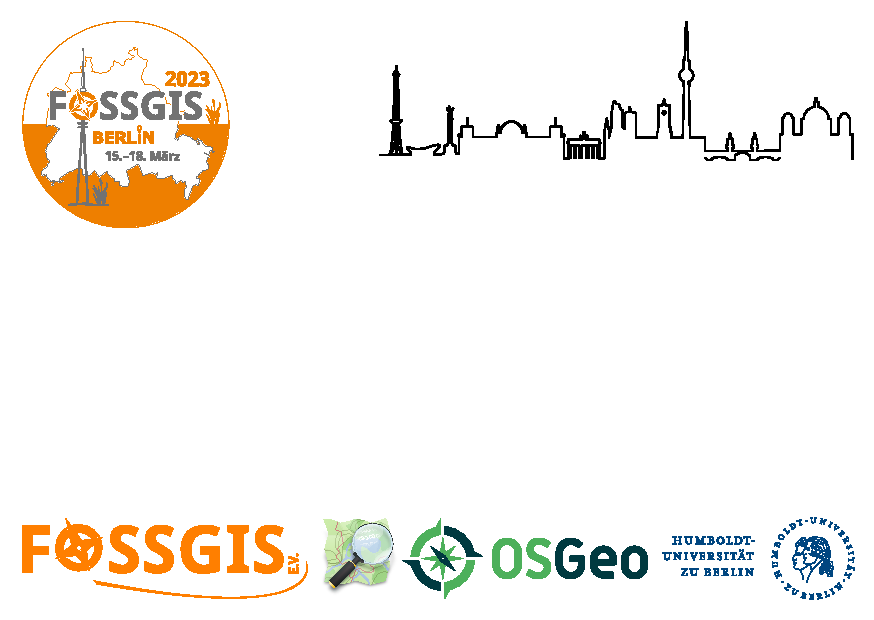
\includegraphics[width=10.5cm]{../imgs/fossgis2023_background.pdf}}
\put(7,34){
  %\scalebox{2}{\textbf{#1}}
  % in der \parbox werden auch lange namen umgebrochen
  \parbox{10cm}{
   % dezente Farbe, damit diese infos nicht auf die Vorderseite durchscheinen
    \color{gray} 
    %%Nachname,Vorname,Ticket,TShirt,TBand,TListe,AV,Mittag,WS,EX,OSM
  	Name: #1, #2 \\
  	Ticket: #3 \\
  	T-Shirt: #4
  	
  }
  }
}}


\begin{document} 
\DTLsetseparator{;}
\DTLloaddb{CSV}{bin/pretix.csv}
\DTLsort{Nachname}{CSV}
%Nachname,Vorname,Ticket,TShirt,TBand,TListe,AV,Mittag,WS,EX,OSM
\DTLforeach{CSV}{\vorname=Vorname,\nachname=Nachname,\type=Ticket,\tshirt=TShirt,
\tband=TBand, \tliste=TListe,\av=AV,\mittag=Mittag,\ex=EX,\osm=OSM}
%\DTLforeach{CSV}{\person=Name,\nickname=268184}
{
 %%Nachname,Vorname,Ticket,TShirt,TBand,TListe,AV,Mittag,WS,EX,OSM
  \schildinnen{\nachname}{\vorname}{\type}{\tshirt}
  %{\type}
  %{\tshirt}{\tband}{\tliste}	
  %{\av}{\mittag}{\ws}{\ex}{\osm}
  %\schildinnen{\person}{\type}{\shirt}{\count}{\dialoge}{\tagungsband}
  \ticket{}
} 
\end{document} 
